%%%%%%%%%%%%%%%%%%%%%%%%%%%%%%%%%%%%%%%%%
% Wenneker Article
% LaTeX Template
% Version 2.0 (28/2/17)
%
% This template was downloaded from:
% http://www.LaTeXTemplates.com
%
% Authors:
% Vel (vel@LaTeXTemplates.com)
% Frits Wenneker
%
% License:
% CC BY-NC-SA 3.0 (http://creativecommons.org/licenses/by-nc-sa/3.0/)
%
%%%%%%%%%%%%%%%%%%%%%%%%%%%%%%%%%%%%%%%%%

%----------------------------------------------------------------------------------------
%	PACKAGES AND OTHER DOCUMENT CONFIGURATIONS
%----------------------------------------------------------------------------------------

\documentclass[12pt, a4paper, twocolumn]{article} % 10pt font size (11 and 12 also possible), A4 paper (letterpaper for US letter) and two column layout (remove for one column)

\usepackage[utf8]{inputenc}
\usepackage[italian]{babel}
\usepackage{float}
\usepackage{wrapfig}
\usepackage{graphicx}
\setcounter{tocdepth}{0}
\usepackage[backend=biber]{biblatex}
\addbibresource{main.bib}

%%%%%%%%%%%%%%%%%%%%%%%%%%%%%%%%%%%%%%%%%
% Wenneker Article
% Structure Specification File
% Version 1.0 (28/2/17)
%
% This file originates from:
% http://www.LaTeXTemplates.com
%
% Authors:
% Frits Wenneker
% Vel (vel@LaTeXTemplates.com)
%
% License:
% CC BY-NC-SA 3.0 (http://creativecommons.org/licenses/by-nc-sa/3.0/)
%
%%%%%%%%%%%%%%%%%%%%%%%%%%%%%%%%%%%%%%%%%

%----------------------------------------------------------------------------------------
%	PACKAGES AND OTHER DOCUMENT CONFIGURATIONS
%----------------------------------------------------------------------------------------

\usepackage[italian]{babel} % English language hyphenation

\usepackage{microtype} % Better typography

\usepackage{amsmath,amsfonts,amsthm} % Math packages for equations

\usepackage[svgnames]{xcolor} % Enabling colors by their 'svgnames'

\usepackage[hang, small, labelfont=bf, up, textfont=it]{caption} % Custom captions under/above tables and figures

\usepackage{booktabs} % Horizontal rules in tables

\usepackage{lastpage} % Used to determine the number of pages in the document (for "Page X of Total")

\usepackage{graphicx} % Required for adding images

\usepackage{enumitem} % Required for customising lists
\setlist{noitemsep} % Remove spacing between bullet/numbered list elements

\usepackage{sectsty} % Enables custom section titles
\allsectionsfont{\usefont{OT1}{phv}{b}{n}} % Change the font of all section commands (Helvetica)

%----------------------------------------------------------------------------------------
%	MARGINS AND SPACING
%----------------------------------------------------------------------------------------

\usepackage{geometry} % Required for adjusting page dimensions

\geometry{
	top=1cm, % Top margin
	bottom=1.5cm, % Bottom margin
	left=2cm, % Left margin
	right=2cm, % Right margin
	includehead, % Include space for a header
	includefoot, % Include space for a footer
	%showframe, % Uncomment to show how the type block is set on the page
}

\setlength{\columnsep}{7mm} % Column separation width

%----------------------------------------------------------------------------------------
%	FONTS
%----------------------------------------------------------------------------------------

\usepackage[T1]{fontenc} % Output font encoding for international characters
\usepackage[utf8]{inputenc} % Required for inputting international characters

\usepackage{XCharter} % Use the XCharter font

%----------------------------------------------------------------------------------------
%	HEADERS AND FOOTERS
%----------------------------------------------------------------------------------------

\usepackage{fancyhdr} % Needed to define custom headers/footers
\pagestyle{fancy} % Enables the custom headers/footers

\renewcommand{\headrulewidth}{0.0pt} % No header rule
\renewcommand{\footrulewidth}{0.4pt} % Thin footer rule

\renewcommand{\sectionmark}[1]{\markboth{#1}{}} % Removes the section number from the header when \leftmark is used

%\nouppercase\leftmark % Add this to one of the lines below if you want a section title in the header/footer

% Headers
\lhead{} % Left header
\chead{\textit{\thetitle}} % Center header - currently printing the article title
\rhead{} % Right header

% Footers
\lfoot{} % Left footer
\cfoot{} % Center footer
\rfoot{\footnotesize Page \thepage\ of \pageref{LastPage}} % Right footer, "Page 1 of 2"

\fancypagestyle{firstpage}{ % Page style for the first page with the title
	\fancyhf{}
	\renewcommand{\footrulewidth}{0pt} % Suppress footer rule
}

%----------------------------------------------------------------------------------------
%	TITLE SECTION
%----------------------------------------------------------------------------------------

\newcommand{\authorstyle}[1]{{\large\usefont{OT1}{phv}{b}{n}\color{DarkRed}#1}} % Authors style (Helvetica)

\newcommand{\institution}[1]{{\footnotesize\usefont{OT1}{phv}{m}{sl}\color{Black}#1}} % Institutions style (Helvetica)

\usepackage{titling} % Allows custom title configuration

\newcommand{\HorRule}{\color{DarkGoldenrod}\rule{\linewidth}{1pt}} % Defines the gold horizontal rule around the title

\pretitle{
	\vspace{-30pt} % Move the entire title section up
	\HorRule\vspace{10pt} % Horizontal rule before the title
	\fontsize{32}{36}\usefont{OT1}{phv}{b}{n}\selectfont % Helvetica
	\color{DarkRed} % Text colour for the title and author(s)
}

\posttitle{\par\vskip 15pt} % Whitespace under the title

\preauthor{} % Anything that will appear before \author is printed

\postauthor{ % Anything that will appear after \author is printed
	\vspace{10pt} % Space before the rule
	\par\HorRule % Horizontal rule after the title
	\vspace{20pt} % Space after the title section
}

%----------------------------------------------------------------------------------------
%	ABSTRACT
%----------------------------------------------------------------------------------------

\usepackage{lettrine} % Package to accentuate the first letter of the text (lettrine)
\usepackage{fix-cm}	% Fixes the height of the lettrine

\newcommand{\initial}[1]{ % Defines the command and style for the lettrine
	\lettrine[lines=3,findent=4pt,nindent=0pt]{% Lettrine takes up 3 lines, the text to the right of it is indented 4pt and further indenting of lines 2+ is stopped
		\color{DarkGoldenrod}% Lettrine colour
		{#1}% The letter
	}{}%
}

\usepackage{xstring} % Required for string manipulation

\newcommand{\lettrineabstract}[1]{
	\StrLeft{#1}{1}[\firstletter] % Capture the first letter of the abstract for the lettrine
	\initial{\firstletter}\textbf{\StrGobbleLeft{#1}{1}} % Print the abstract with the first letter as a lettrine and the rest in bold
}

%----------------------------------------------------------------------------------------
%	BIBLIOGRAPHY
%----------------------------------------------------------------------------------------

% \usepackage[backend=bibtex,style=authoryear,natbib=true]{biblatex} % Use the bibtex backend with the authoryear citation style (which resembles APA)

\addbibresource{example.bib} % The filename of the bibliography

\usepackage[autostyle=true]{csquotes} % Required to generate language-dependent quotes in the bibliography
 % Specifies the document structure and loads requires packages

% \usepackage{textcomp}

%----------------------------------------------------------------------------------------
%	ARTICLE INFORMATION
%----------------------------------------------------------------------------------------

\title{Sound of Data} % The article title

\author{
  \authorstyle{
    % DO NOT TOUCH HSPACEs!! @Momo
    Riccardo Cervero \hspace{25pt} 794126 \\  % x + 4
    Marco Ferrario \hspace{44pt}  795203 \\   % x + 23
    Pranav Kasela \hspace{46.5pt} 846965 \\   % x + 25.5
    Federico Moiraghi \hspace{21pt} 799735    % x
  } % Authors
  \newline\newline
  \institution{Università degli Studi di Milano Bicocca}
}

\date{Anno Accademico 2018/19} % Add a date here if you would like one to appear underneath the title block, use \today for the current date, leave empty for no date

%----------------------------------------------------------------------------------------

\begin{document}

\maketitle % Print the title

\thispagestyle{firstpage} % Apply the page style for the first page (no headers and footers)

%----------------------------------------------------------------------------------------
%	ABSTRACT
%----------------------------------------------------------------------------------------

\lettrineabstract{Obiettivo del progetto è analizzare la discussione mediatica sul social network Twitter, studiandone in tempo reale l'andamento nell'ambito musicale, presente e passato.
Lo scopo è  verificare la presenza di variazioni all'interno del ciclo giornaliero e quella delle comunità digitali, e le relative interconnessioni.
Il presente lavoro può essere di aiuto nella costruzione di sistemi di raccomandazione interni a Twitter (quali pagine consigliate) e nella programmazione di BOT, a scopo pubblicitario, che intendano entrare in una discussione mediatica già presente (ovvero argomenti di tendenza) per inserire i propri messaggi.}
\newpage

\tableofcontents
\hfill
\newpage

%----------------------------------------------------------------------------------------
%	ARTICLE CONTENTS
%----------------------------------------------------------------------------------------
\part{Introduzione}
I traguardi posti dal progetto \textit{Sound of Data}\footnote{\url{https://github.com/pkasela/Sound-of-Data}}, hanno innanzitutto richiesto l'uso di uno \textit{knowledge graph} adeguato alla materia: scaricato un \textit{dump} di \url{musicbrainz.org}, versione \textit{semantic web} di \url{last.fm}, disponibile pubblicamente in formato \verb|.tsv| (\textit{Tabular Separated Values}), si è provveduto ad importarlo all'interno di Apache Hadoop\footnote{\url{https://hadoop.apache.org}} per effettuare una rapida pulizia preliminare.
Fatto ciò, i dati sono stati importati in Neo4J\footnote{\url{https://neo4j.com}}, grazie al pratico programma \verb|neo4j-import|, in modo da costruire lo \textit{knowledge graph} richiesto per l'analisi dei \textit{tweet}, raccolti ed analizzati in tempo reale grazie ad Apache Kafka\footnote{\url{https://kafka.apache.org}}: grazie ad un efficiente plug-in\footnote{\url{https://github.com/neo4j-contrib/neo4j-streams}} che permette l'uso di \textit{Neo4j} come \textit{Consumer}, il singolo tweet è archiviato nativamente in uno schema a grafo.
Durante il processo di \textit{streaming}, questi subiscono varie operazioni di \textit{preparation} e vengono filtrati da un rudimentale strumento di \textit{instance matching}.

Dopo la complessa fase di gestione e raccolta dei dati, è stato possibile condurre un'analisi finale sulle dinamiche della discussione musicale instauratesi fra i singoli utenti all'interno di comunità, astratte ed estremamente mutevoli, e sulle relazioni, più o meno intense, esistenti fra di esse.
Le progressiva composizione  dei nodi, rappresentanti i \textit{tweet} all'interno del grafo, è studiata ad intervalli regolari, corrispondenti a quattro fasce orarie relative al mattino, pomeriggio, sera e notte.
Si è preferito adoperare tale ciclo giornaliero, anziché un più ampio ciclo settimanale o addirittura mensile, per due ragioni precise.
Innanzitutto, questo garantisce una più facile interpretazione: risulta di estremo interesse osservare i trend ricorrenti nei vari momenti della giornata, piuttosto che riferiti all'arco settimanale.
Inoltre, il ciclo giornaliero ha il vantaggio di non risentire della distorsione provocata dagli eventi, previsti o meno.
Infatti, essendo gli eventi in grado di assorbire l'interesse della gran parte dell'opinione pubblica per interi giorni e settimane, questi penalizzano l'analisi e concentrano tutti gli utenti verso un numero limitato di argomenti musicali.
Due esempi riguardanti tale problematica, e le sue conseguenze negative, possono essere citati per quanto concerne il genere \textit{drone}, per cui, durante il periodo di raccolta, si sono succeduti due eventi particolarmente rilevanti: il primo riguarda l'abbattimento di un drone americano in territorio Iraniano, causando nuove tensioni fra i due Paesi\footnote{\url{http://www.ansa.it/sito/notizie/mondo/mediooriente/2019/06/20/iran-pasdaran-abbattuto-drone-usa_b8922ea0-e61c-436b-8f66-60f3be32ed21.html}}, mentre il secondo consiste in uno spettacolo di droni luminosi a Torino\footnote{\url{https://www.guidatorino.com/eventi-torino/san-giovanni-torino-droni-2019/}} per la festa patronale.

Raccogliendo l'attenzione di centinaia di utenti, i due eventi e la polisemia della parola hanno fatto sì che la comunità di ascoltanti il genere musicale \textit{drone} fosse sproporzionatamente più grande rispetto alle altre nei giorni degli eventi; ma tale distorsione è stata diluita dalla divisione in fasce orarie e dalla moltitudine dei giorni in cui è stata effettuata la raccolta dati.
\hfill
\newpage


\part{Costruzione dello \textit{knowledge graph}}

\section{Data Cleaning con Python e Pig}
I dati sono stati scaricati dal sito di musicbrainz attraverso lo script python \verb|get_data.py|\footnote{\url{https://github.com/pkasela/Sound-of-Data/blob/master/musicbrainz_data/Data_Cleaning/get_data.py}} che cerca sul sito l'ultima versione del database e la scarica col comando \verb|wget| dei sistemi Unix.
Decompressa quindi la cartella con il dump del database e selezionati solamente i file necessari allo scopo, vengono eseguite delle operazioni \verb|cat-sed| per effettuare una rapida pulizia preliminare (la gestione dei valori nulli \verb|\N|).
È stata salvata inoltre una lista di generi musicali, già presente in una pagina HTML del sito, tramite uno \textit{scraper}, che ne analizza l'elenco per importarla in Python.

%%%%%%
%%%%%%%%%%%
%%%%%%%%%%%%%%%%
%%%% Ma lo schema iniziale va messo?
%%%% Io dico di no al massimo lo schema finale
%%%%%%%%%%%%%%%%
%%%%%%%%%%%
%%%%%%

I file sono stati successivamente importati e processati all'interno del \textit{file system} HDFS.
Nel dettaglio, questa fase viene eseguita attraverso l'utilizzo di Apache Pig, piattaforma atta all'elaborazione di grosse quantità di dati.
La decisione di utilizzare Pig anzichè SQL dipende principalmente dalle migliori prestazioni del primo nella fase di caricamento, e dalla maggiore versatilità della suite Hadoop per la fase di elaborazione.
L'\textit{engine} adoperato in combinazione con Pig non è MapReduce ma Tez: costruito sopra YARN\cite{apacheTez}, migliora drasticamente le prestazioni mantenendo la stessa scalabilità poiché evita alcune fasi di scrittura di risultati parziali sull'HDFS (vedere Figura \ref{fig:Hadoop} per maggiori dettagli\cite{tez}).

\begin{figure*}
  \centering
  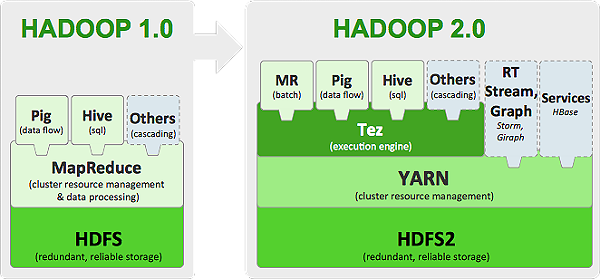
\includegraphics[width=\linewidth]{hadoop2.png}
  \caption{Differenza architteturale di HADOOP 1.0 con MapReduce rispetto alla versione 2.0 con Tez.}
  \label{fig:Hadoop}
\end{figure*}

Più precisamente, la velocità di esecuzione è ottenuta grazie all'invio diretto dei dati da un processo all'altro, evitando la scrittura all'interno del file system, eccezion fatta per i \textit{checkpoints}.
Inoltre, la definizione del \textit{job} sfrutta i \textit{Directed Acyclic Graph}, dove i vertici rappresentano gli step del processo e gli archi la connessione tra i vertici \textit{Producer} e \textit{Consumer} (come mostrato in figura\cite{apacheTez, tez}).

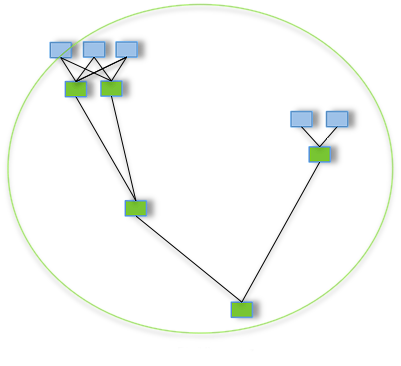
\includegraphics[width=0.9\linewidth]{tez.png}

Conclusa la fase di pulizia, i dati sono trasferiti all'esterno di HDFS sul filesystem reale, unendo i risultati di Pig  mediante il comando \textit{cat} di \textit{Unix}. 
A questo punto i dati sono pronti per essere importati in Neo4j.

%%%%%%
%%%%%%%%%%%
%%%%%%%%%%%%%%%%
%%%% Conviene mettere lo schema finale delle tabelle (dopo lo metto)
%%%%%%%%%%%%%%%%
%%%%%%%%%%%
%%%%%%

\section{Import dei dati in Neo4J}
In seguito, il risultato dell'elaborazione svolta da Pig viene caricato all'interno del \textit{DBMS Neo4j} usando il comando \verb|neo4j-import|\cite{neo4jImport} e indicizzando i \textit{gid} delle varie entità, in modo da velocizzare la ricerca da svolgere successivamente.

Il risultato è un grafo dal peso approssimativo di 5Gb contenente i vari artisti, i relativi album e le relative case discografiche, collegati tra di loro in modo opportuno.
Si è preferito ridurre la capillarità del database evitando di inserire le singole canzoni contenute negli album, sia perché una simile precisione sarebbe stata difficile da gestire in fase di analisi, sia a causa della mancanza nel dump del database di tale informazione (comunque presente nella versione online), che avrebbe richiesto un tempo superiore alla settimana (dovuto perlopiù alla latenza supportata dal sito) per poter essere recuperata.


\hfill
\newpage
\part{Streaming dei tweet}
\section{Elaborazione mediante Apache Kafka}
%
Nella fase di gestione e analisi in tempo reale, i \textit{tweet} vengono filtrati ed elaborati mediante una sequenza di operazioni, attraverso una \textit{pipeline} costituita dalla concatenazione di due coppie di processi \textit{Producer} e \textit{Consumer}.
L'architettura di elaborazione in \textit{streaming} è stata così configurata per garantire una maggiore scalabilità ed una migliore performance, riuscendo a reggere volumi di \textit{tweet} in ingresso maggiori.
Questi vengono estratti grazie all'API \textit{Tweepy}\footnote{\url{https://tweepy.readthedocs.io/en/latest/}} per Python, utilizzando come parole chiave di ricerca una selezione di 400 generi musicali fra i 419 ottenuti dallo scraping della pagina \url{'https://musicbrainz.org/genres'}, e ricevendo soltanto i testi pubblicati in lingua italiana.

Quindi i \textit{tweet} vengono inviati ad una prima Topic come messaggi di un \textit{Producer} di Kafka, inizializzato mediante la libreria \textit{Kafka-python}\footnote{\url{https://kafka-python.readthedocs.io/en/master/}}. 
All'interno di un secondo file\footnote{\url{https://github.com/pkasela/Sound-of-Data/blob/master/NL/Kafka_Producer_2.py}}, associato ad un nuovo processo Producer, dunque ad una seconda Topic connessa in \textit{streaming} con la precedente, il JSON grezzo che costituisce ciascun \textit{tweet} in ingresso viene processato in vari step dalla funzione \verb|tweet_preparations|.

La prima fase coincide con l'estrazione dello \textit{screen name} dell'utente, del contenuto postato e dell'ora e data precisa di pubblicazione. 
In particolare, il testo viene modificato in modo da rendere leggibili i caratteri speciali e i cosiddetti \textit{escape characters}. 

La seconda fase sfrutta l'API di \textit{Botometer}\footnote{\url{https://rapidapi.com/OSoMe/api/botometer/details}} per calcolare la probabilità - definita \textit{score} - che un profilo sia in realtà gestito da un BOT, osservandone il comportamento passato.
Poiché i profili gestiti in modo automatico alterano, spesso fortemente, la discussione mediatica aumentando arbitrariamente il flusso di determinati contenuti, si è deciso di non archiviare i \textit{tweet} appartenenti a tali profili. 
Nel dettaglio, se lo score associato all'utente di ogni \textit{tweet} supera una soglia (fissata arbitrariamente al $90\%$), lo \textit{screen name} viene memorizzato all'interno di una \textit{blacklist}, altrimenti viene smistato in una \textit{whitelist}, in modo che il programma possa riconoscere più velocemente ogni profilo ed evitare inutili ricalcoli.
In questo modo, si riduce il numero di richieste fatte all'API, gratuita fino ad un certo volume e poi a pagamento.
Per aumentare ulteriormente l'efficienza di questo processo e garantire la scalabilità, si è scelto di adoperare il \textit{data store Riak}, di tipo \textit{NoSQL Key-Value}, interfacciato per mezzo della propria libreria Python\footnote{\url{https://github.com/basho/riak-python-client}}\cite{riakTutorial}: viene così archiviato lo \textit{score} di ogni utente e la richiesta all'API è effettuata solamente se non si trova la chiave nel database.

La terza fase verifica che il testo contenga entità di rilevo, grazie ad un rudimentale \textit{istance matcher} che tenta di riconoscere le parole riguardanti il contesto musicale, aggiungendo al dizionario prodotto dalle fasi precedenti tre chiavi corrispondenti rispettivamente alla lista di artisti, album o canzoni estratti dal testo analizzato.
Ciò è permesso dall'uso dell'API\footnote{\url{https://python-musicbrainzngs.readthedocs.io/en/v0.6/api/}} fornita dal sito \textit{musicbrainz.org} e basata su Apache Lucene\footnote{\url{https://lucene.apache.org/}}.
Per maggiori dettagli si rimanda alla sezione dedicata.

Ogniqualvolta si verificano le due condizioni note, cioè che l'utente non abbia probabilità elevata di essere un BOT e che il testo pubblicato si riferisca effettivamente al mondo della musica, ciascun risultato della funzione \verb|tweet_preparations| è ricodificato e passato come messaggio al secondo \textit{Producer} di \textit{Apache Kafka} - menzionato in precedenza - che effettuerà l'invio del dato finale alla \textit{topic} nominata \textit{KafkaTopic}. 
Grazie all'utilizzo di questa piattaforma, il flusso di \textit{feed} è gestito in tempo reale, assicurando bassissima latenza e grande scalabilità. 

\section{Consuming dei Tweets in Neo4j}
Uno dei principali vantaggi di \textit{Apache Kafka} consiste nella capacità di connettersi efficientemente a sistemi esterni, garantendo in tal modo la continuità dello \textit{stream} di dati da una fonte - la classe \textit{Listener} adoperata in Python per "ascoltare" i tweet grazie all'API Tweepy - ad una \textit{"landing zone"}, che in questo caso corrisponde al DBMS \textit{Neo4j}. 
Si è scelto di effettuare lo \textit{storage} dei \textit{tweets} in un \textit{GraphDB}, e in particolare \textit{Neo4j} per le sue caratteristiche di estrema scalabilità, efficienza nella gestione dei dati, elevata capacità di adattamento al fenomeno di studio e facile interpretabilità.
L'esportazione diretta dei tweet da \textit{Apache Kafka} all'interno del \textit{data store} avviene grazie a un \textit{plug-in} di \textit{Neo4j}, \textit{"Neo4j Streams Consumer"}.
Questo si configura come un'applicazione che effettua un'ingestione diretta e automatizzata all'interno di \textit{Neo4j}, permettendo la lettura dei dati presenti nella \textit{topic} allo stesso modo di qualsiasi applicazione \textit{Consumer} di \textit{Kafka}.

\textit{Neo4j Streams Consumer} permette all'utente di specificare arbitrariamente relazioni, entità e proprietà in cui i \textit{payloads} di \textit{Apache Kafka}, corrispondenti al JSON di ciascun \textit{tweet} importato, dovranno essere organizzati per costruire progressivamente il grafo.
La struttura di quest'ultimo viene dichiarata attraverso un \textit{Cypher template}, ovvero un insieme di \textit{queries} semantiche di \textit{Cypher}, all'interno di un file di configurazione, che nel caso presentato è \verb|docker-compose.yml|\footnote{\url{https://github.com/pkasela/Sound-of-Data/blob/master/Neo4j\%20\%26\%20kafka/docker-compose\%20configuration.yml}}, poiché il progetto viene eseguito mediante \textit{Docker Desktop}, in quanto quest'ultimo presenta il vantaggio di riuscire a far comunicare automaticamente e in maniera trasparente i containers coinvolti. 
Una volta specificato il \textit{Cypher template}, installato il \textit{plug-in} all'interno del \textit{Docker}, e successivamente montati i container e i relativi collegamenti, la fase di mera esecuzione del progetto avviene mediante la funzione denominata \verb|streams.consume|, la quale crea immediatamente la struttura del grafo come indicato.

Nello specifico, all'arrivo di un \textit{tweet} verranno dunque aggiunti i nodi \verb|Tweet|, \verb|User| ed un terzo che riporterà ora e data di pubblicazione.
Il primo conterrà le \textit{property keys} del testo \verb|text|, e dello \verb|screen_name|. 
Il secondo, invece, conterrà solamente la proprietà \textit{"name"}, che riporta lo \textit{screen name}. 
Tra i primi due nuovi nodi verrà generata la relazione \verb|BELONGS_TO|, ad indicare il profilo di appartenenza di ciascun post, mentre \verb|User| sarà connesso alla data e ora di pubblicazione da un \textit{edge} etichettato come \verb|Twitted|.

Inoltre il programma effettua automaticamente un'operazione di \textit{merge} della coppia appena generata coi nodi già presenti nel grafo: quando è individuato l'\verb|id| di un'entità presente nel testo, il software collega il nodo del tweet all'entità con una relazione \verb|TALKS_ABOUT|.
L'entità presente su musicbrainz viene collegata al proprio genere musicale, così da fare da tramite tra i nodi riguardanti genere e \textit{tweet}, punto focale del progetto.

Dunque il grafo conterrà una serie di nodi utente, raggruppati in comunità attorno ad artisti o generi a seconda dell'oggetto dei propri \textit{tweet}.
Grazie a questa semplice struttura, l'analisi può avvenire già in maniera grafica e trasparente, e l'utente è in grado di distinguere la grandezza di queste comunità, ed intendere quali e quanto intensi legami esistano fra di esse.
Per ottenere queste informazioni, è infatti sufficiente scaricare un \textit{dump} del grafo a intervalli regolari e confrontare i vari risultati.
Il risultato finale, dall'interfaccia web di \textit{Neo4j}, apparirà come nella seguente figura:
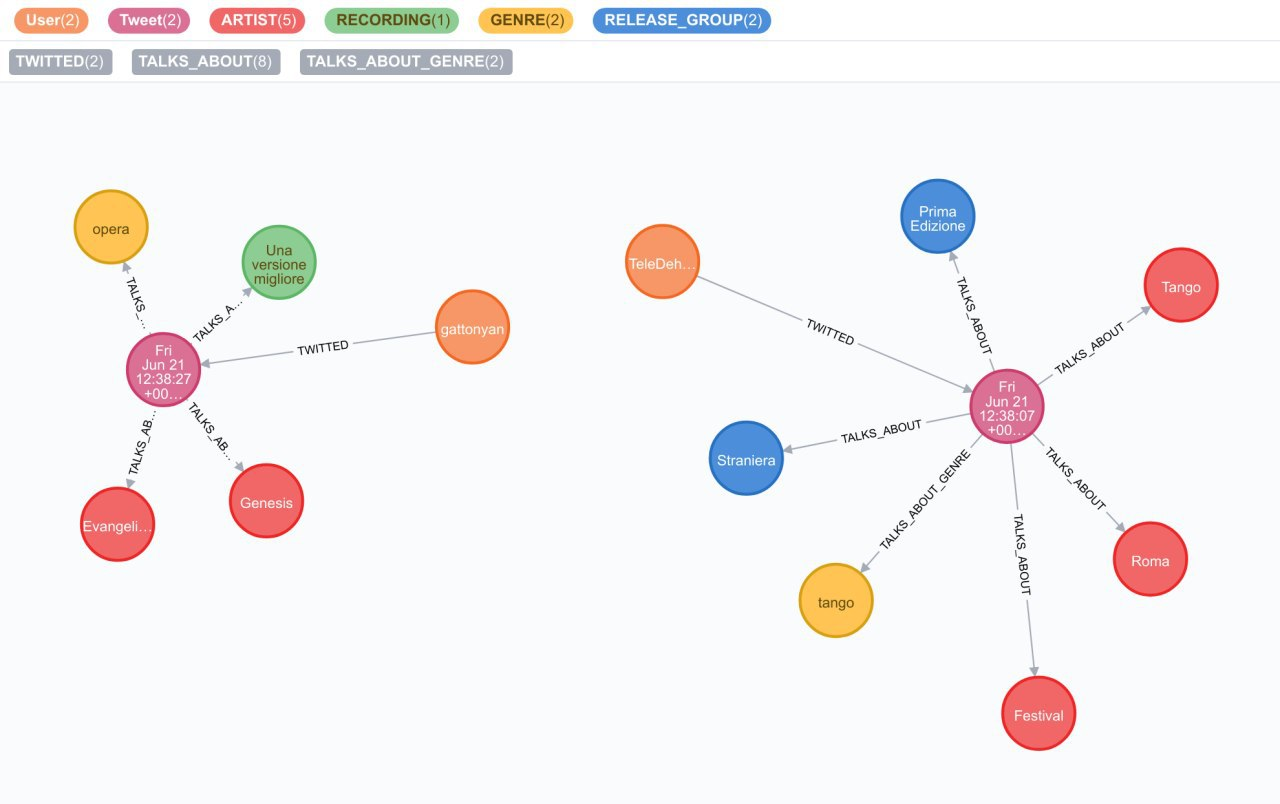
\includegraphics[width=\linewidth]{small_graph.png}

Invece, la composizione dei cluster, cioè delle comunità ben separate, verrà mostrata come di seguito:

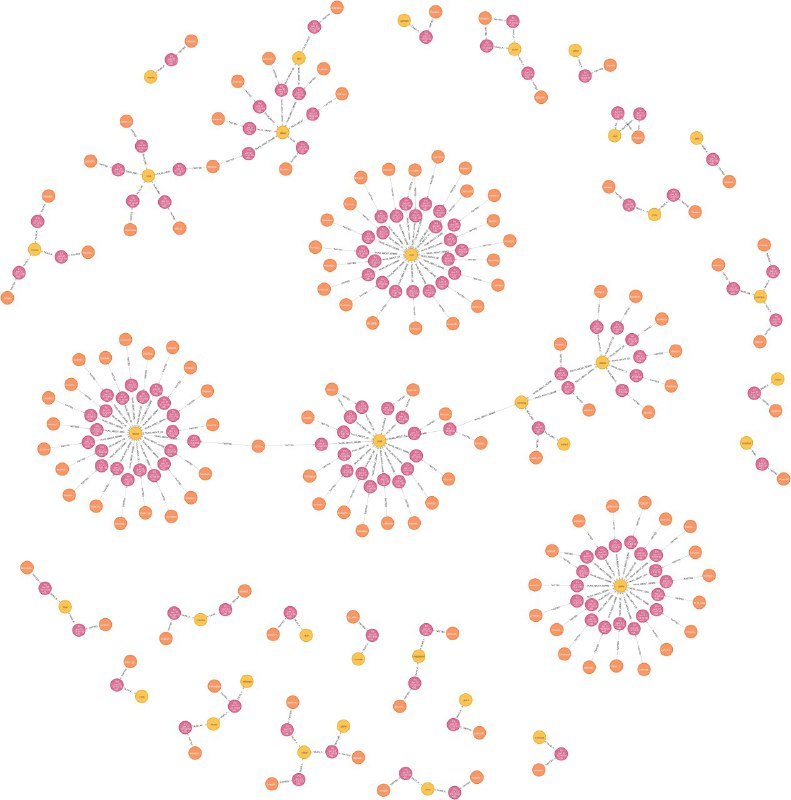
\includegraphics[width=\linewidth]{big_graph.png}

\section{Riconoscimento delle istanze nel testo}
Data la quantità e qualità dei dati, si è deciso di costruire un strumento di \textit{instance matching} creato \textit{ad hoc} per i tweet: le API disponibili basate su \textit{deep learning} sono spesso allenate su altri tipi di testo (articoli di giornale o opere letterarie) e spesso non offrono una velocità adeguata per l'analisi in tempo reale.
Il problema della qualità del testo è fondamentale: serve uno strumento che riesca ad analizzare il testo e a trovare le entità corrispondenti senza bisogno di contestualizzazione.
Per tale scopo, filtrati già in partenza i tweet grazie a parole chiave a tema musicale, si costruisce un modello che identifichi le istanze restituendone gli \verb|id| grazie all'API di musicbrainz disponibile per Python.

\subsection{Identificazione delle entità}
Le entità sono riconosciute non mediante \textit{machine learning} ma grazie a semplici stratagemmi linguistici e l'aiuto di un correttore ortografico.
Prima di tutto il testo del tweet è ripulito da eventuali abbreviazioni gergali (che vengono sostituite dalla propria forma estesa), link e caratteri speciali.
Subito dopo sono ricercate le parole nel testo che non risultano essere italiane: analizzando tweet in lingua italiana, il cui tema è sicuramente musicale, si presume che una stringa in lingua diversa abbia una certa importanza; ciò è fatto sia analizzandone l'ortografia sia verificando con un'espressione regolare che le parole rispecchino la regola di costruzione delle sillabe in italiano\footnote{Una sillaba in italiano è composta da un massimo di tre consonanti iniziali, vocale ed eventuale consonante finale\cite{linguistica}.}.
In tal caso, la parola è un sostantivo di una lingua straniera e come tale quindi degna di attenzione.
Infine sono analizzate le parole la cui iniziale è maiuscola, col supporto di un albero sintattico (costruito grazie ad un programma esterno, \verb|TreeTagger|\footnote{\url{https://www.cis.uni-muenchen.de/~schmid/tools/TreeTagger/}}, interfacciato con Python grazie ad un wrapper\footnote{\url{https://perso.limsi.fr/pointal/doku.php?id=dev:treetaggerwrapper}} fornito dagli stessi sviluppatori) per verificare che siano nomi propri.

Inoltre, grazie all'uso della punteggiatura e delle preposizioni, si tenta di stabilire se la presunta entità sia un artista o un'opera, verificando poi con certezza confrontando con lo \textit{knowledge graph}. \newline

Tramite le API di musicbrainz, attraverso una serie di funzioni \verb|search|, è possibile consultare il database online utilizzando la tecnologia \textit{Lucene}.
Analizzate le entità e tentato di stabilire cosa rappresentino, si interroga la base di conoscenza con le funzioni \verb|search_artists| e \verb|search_recordings| per le entità riconosciute rispettivamente come artisti e opere, a cui si aggiunge \verb|search_release_groups| (funzione relativa alla ricerca degli album), per quelle di tipologia incerta.
Per verificare la corrispondenza tra entità e risultati di ricerca, si è scelta la politica di accettare il risultato la cui similarità coseno è maggiore, a patto che superi una soglia arbitraria di $0.95$.
Inoltre, per aumentare la precisione, si sono incrociati i risultati parziali delle ricerche per testare se nello stesso testo compaia l'opera accompagnata dal proprio autore.

\subsection{Prestazioni del modello e margini di miglioramento}
La problematica principale emersa nella costruzione del modello è stata la corretta attribuzione dell'entità nei casi di omonimia: questi casi infatti sono molto frequenti tra canzoni ed album relativi ad artisti differenti ed è quindi possibile che il risultato ottenuto non sia quello desiderato.

Inoltre, nonostante il modello offra una buona \textit{performance} nella selezione dei testi riferiti al mondo musicale e nel riconoscimento delle istanze nel testo, continua a presentare alcune imperfezioni.
Un primo difetto deriva dalla difficoltà nella gestione dei casi polisemici: alcuni nomi di genere (in particolare \textit{drone}, \textit{dance}, \textit{club} e \textit{opera}) sono polisemici, distorcendo i valori dell'analisi.
Il programma utilizzato è troppo rudimentale per distinguere il contesto e quindi mostra numerosi falsi positivi: il termine \textit{club} in particolare viene spesso citato all'interno di testi riguardanti qualsiasi tipo di associazione; la parola \textit{drone}, come già accennato nell'introduzione, indica, nella maggior parte dei casi, l'aeromobile; l'espressione \textit{dance} è frequentemente slegata alla musica e \textit{opera} possiede troppi significati estranei al contesto in questione.

Un'altra problematica, non legata al modello ma a \verb|tweepy|, è sorta dopo aver rilevato alcuni \textit{tweet} in lingua straniera (perlopiù spagnola) che citavano il termine \textit{trap} senza riferirsi al genere musicale.

Pertanto, il modello raggiunge buoni risultati nell'ambito di questo progetto, rendendo comunque necessari ulteriori tentativi di miglioramento della sua capacità di riconoscere il contesto all'interno del quale le parole vengono citate.

\section{Scalabilità}
È facile ottenere una buona scalabilità orizzontale del programma grazie alla dimensione fissa (relativamente contenuta) della base di conoscenza e all'architettura dei singoli componenti: Kafka e Riak infatti permettono nativamente la gestione di più \textit{cluster} nel database, distribuendo i dati in modo efficiente.
L'unico inconveniente in cui è possibile imbattersi è l'eccessivo aumento dei \textit{tweet} nel tempo: per risolvere questo problema è possibile replicare la base di conoscenza su ogni nodo e in seguito smistare i messaggi tra questi (secondo un criterio prefissato).
La struttura a grafo infatti non è frammentabile, ma necessaria principalmente per facilitare la consultazione della base di conoscenza (lo \textit{knowledge graph}) e ottimizzare la gestione dei collegamenti con le entità nei testi.
Dunque frammentare le informazioni riguardanti gli utenti è un ottimo sistema per dividere il carico di lavoro fra i \textit{cluster}.

In alternativa, è disponibile una versione a pagamento di Neo4J\cite{neo4jEnterprise} che permette una divisione multi-cluster del database: in questo modo ogni componente del progetto è scalabile orizzontalmente in modo nativo.

Per comodità, tuttavia, il lavoro svolto è stato fatto interamente sulla stessa macchina, grazie anche al basso volume dei \textit{tweet} ricevuti (dell'ordine di grandezza del Megabyte): ciò ha permesso di evitare tale problematica.

\hfill
\newpage
\hfill
\newpage
\part{Visualizzazioni dei dati}
\section{Distribuzione dei principali generi musicali nelle quattro fasce orarie}
La prima visualizzazione consiste nella tipologia \textit{barchart}, realizzata con il software \textit{Tableau}.
In ascissa, il grafico raccoglie i principali quarantasette generi musicali estratti dall'analisi delle pubblicazioni avvenute tra il 21 e il 28 giugno, ordinati in senso crescente secondo la frequenza assoluta totale. 
L'ordinata, invece, è segmentata nelle quattro sezioni dedicate rispettivamente al periodo notturno, mattutino, pomeridiano e serale. 
In ogni sezione, la dimensione della barra corrisponde al numero di volte in cui il dato genere è stato menzionato durante la specifica fascia oraria.
Pertanto, sommando verticalmente i valori, si otterrà la dimensione globale associata ad ogni genere.

Tuttavia, sulle misure parziali, relative quindi al singolo intervallo temporale, è stato necessario effettuare un filtro: dato che si è deciso di mantenere la scala naturale dei valori, le barre associate alle frequenze minori di 5 in valore assoluto sono state omesse, per evitare che l'ascissa risultasse carica di un eccessivo numero di generi, peggiorando la consultazione.
In ogni caso, avrebbero assunto dimensioni troppo piccole per poter essere visibili.

Perciò, considerando la sola variabile della frequenza assoluta, dal punto di vista dell'"\textit{overview}" il fruitore è in grado di individuare la distribuzione dei vari generi, e intuire immediatamente quali siano i più presenti. 
Ad esempio, è chiaro come \textit{"dance"} sia il genere comparso più volte durante il pomeriggio, o ancora \textit{"rave"} il più presente durante la mattina. 
Inoltre, è possibile notare come la notte rappresenti ovviamente il periodo meno produttivo per quanto riguarda il numero di pubblicazioni, e, viceversa, come la mattina accolga un flusso di tweet a tema musicale nettamente maggiore. 
Infine, la componente dell'interattività permette di ottenere i dati di ogni singolo genere, approfondendo le sue caratteristiche e valutando la sua disposizione nell'arco della giornata.

Una seconda variabile è stata aggiunta al grafico: la misura di appartenenza di ogni genere musicale ad ogni fascia oraria, ovvero la tendenza percentuale di ogni genere a comparire in una particolare fascia oraria, rispetto al totale dei tweet che lo riguardano. 
Quanto maggiore è la concentrazione delle citazioni ad esso riferite in uno dei quattro periodi, tanto superiore sarà il suo grado di appartenenza al dato intervallo temporale. 
L'indice, che, essendo una percentuale, accoglie valori da zero a uno, è rappresentato attraverso il dettaglio della saturazione del colore blu in ogni barra.
A questo punto, il fruitore non è soltanto in grado di percepire visivamente la presenza di un particolare genere, ma anche il suo diverso legame con i quattro momenti della giornata. 
Con l'obiettivo di evidenziare i valori più interessanti sotto questo punto di vista, le prime tre maggiori percentuali di appartenenza, per ogni intervallo temporale, vengono specificate sopra le relative barre. 
In più, il massimo e il minimo vengono descritti testualmente. È così possibile osservare come la musica classica rappresenti il genere musicale più specifico, poichè citata nel 77\% dei casi durante la sera.

Una sezione speciale del grafico, sul lato destro, viene dedicata alle quattro tipologie musicali più presenti. 
Innanzitutto, questo \textit{zoom} permette al fruitore di cogliere in maniera migliore la differenza e la composizione interni dei quattro maggiori elementi, potendo effettuare un miglior confronto visivo. 
In secondo luogo, la rappresentazione dell'estremo inferiore e superiore dell'intervallo di confidenza, calcolato al 95\%, permette di capire se e quali differenze fra le frequenze assolute siano significative, in modo da attribuire una validità statistica ai parametri estratti dalla distribuzione campionaria. 
Nel dettaglio, il numero di volte in cui la categoria \textit{"dance"} è comparsa all'interno delle dinamiche della discussione su Twitter appare significativamente maggiore rispetto a quello relativo a \textit{"rave"}, ma non rispetto a \textit{"jazz"} e \textit{"rock"}. 

\section{Frequenza assoluta dei generi nella discussione a tema musicale}
Un approfondimento grafico sulla presenza delle principali categorie all'interno delle dinamiche della discussione virtuale è offerto mediante realizzazione di un \textit{wordcloud} costruito con \textit{Python}. 
Grazie alla semplicità di questa visualizzazione, l'osservatore può percepire visivamente la differenza fra le varie grandezze, ordinate a comporre la forma di una nota musicale.

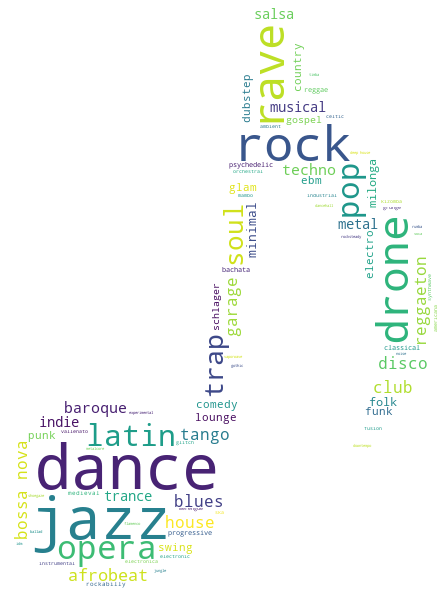
\includegraphics[width=\linewidth]{music_word_cloud.png}

\section{Critiche alla visualizzazione e margini di miglioramento}
Le critiche poste dal campione di fruitori durante l'osservazione e la valutazione del grafico \textit{barchart} hanno riguardato maggiormente la mancanza di un adeguato livello di intuitività della visualizzazione, dovuta principalmente alla presenza di molti elementi grafici in uno spazio ridotto.
Nonostante ciò, questa problematica non pare aver mai penalizzato gravemente la fruizione del grafico e la comprensione finale dell'oggetto descritto dall'analisi. 
Infatti, durante l'esecuzione di un'attività interattiva - che consisteva nel chiedere di selezionare alcuni generi in base a precise caratteristiche - gli utenti coinvolti sono riusciti in ogni caso a soddisfare correttamente le richieste.

Altro problema riscontrato è l'inserimento degli intervalli di confidenza nel grafico totale: i non addetti al settore hanno trovato di difficile interpretazione la lettura delle barre rosse a indicare i limiti superiori e inferiori.
Pertanto si sono limitati a ignorarne la presenza considerandoli più elementi di disturbo che informativi.

Per quanto riguarda il \textit{wordcloud}, le uniche critiche sono state mosse da persone di età superiore ai 50 anni d'età: tale grafico può risultare una novità e può anche risultare poco intuitivo.
Tuttavia, spiegato il funzionamento, questo è stato particolarmente apprezzato da tutti i fruitori, soprattutto a causa della sua semplicità.

\section{Risultati dei questionari psicometrici}
% introduzione: popolazione degli intervistati, numero e metodologia di ricerca
Per valutare l'efficacia delle due infografiche, sono state intervistate 31 persone mediante un questionario, costruito con Google Form\footnote{\url{https://www.google.com/forms/about/}}, in cui dovevano essere attribuiti dei punteggi da 1 a 6 a cinque caratteristiche, seguiti da un punteggio complessivo.
Inoltre è stata cronometrata la velocità a rispondere ad una semplice domanda (identificare il secondo genere più citato la mattina) a un numero più limitato di persone, per testare l'efficienza del grafico.
Infine, ad un numero ancora più limitato, sono stati chiesti pareri (non strutturati) riguardo l'efficienza del grafico e possibili margini di miglioramento.

\subsection{Punteggi al test psicometrico}
% risultati: violin plot e barplot per mostrare i punteggi medi e la loro distribuzione
I risultati ottenuti dalle interviste sono riassunti da un \textit{violin plot} (Figure \ref{plot:violin} e \ref{plot:violin_fm}), così da avere a colpo d'occhio la distribuzione dei punteggi e il loro valore medio.
\begin{figure*}[p]
  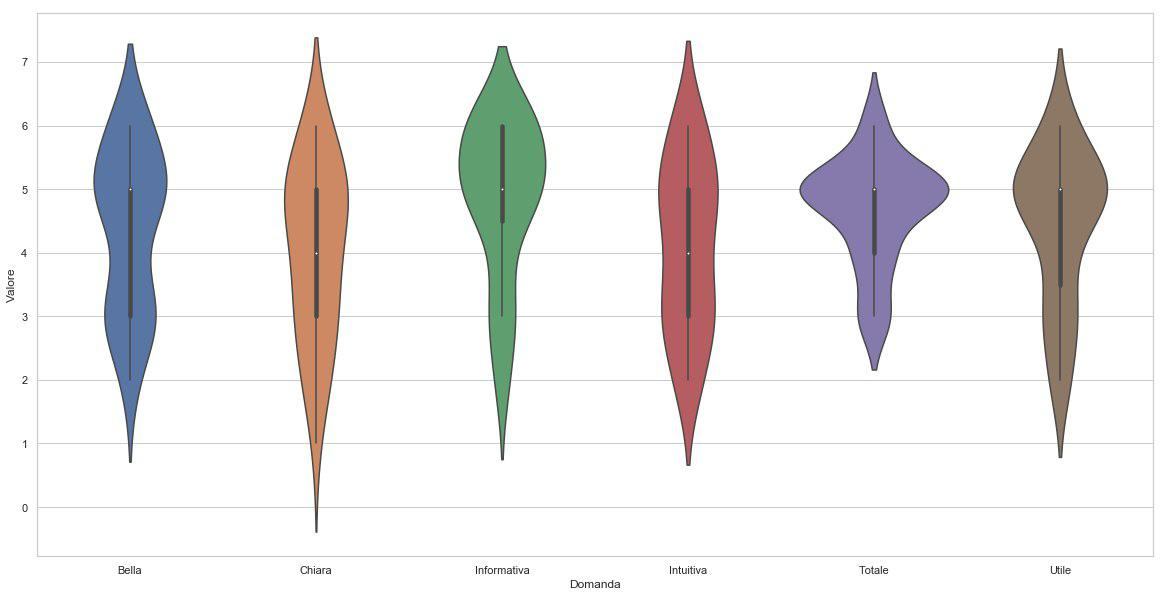
\includegraphics[width=\textwidth]{violin_plot.jpg}
  \caption{Violin plot dei punteggi ottenuti al test in formato aggregato.}
  \label{plot:violin}
\end{figure*}
\begin{figure*}[p]
  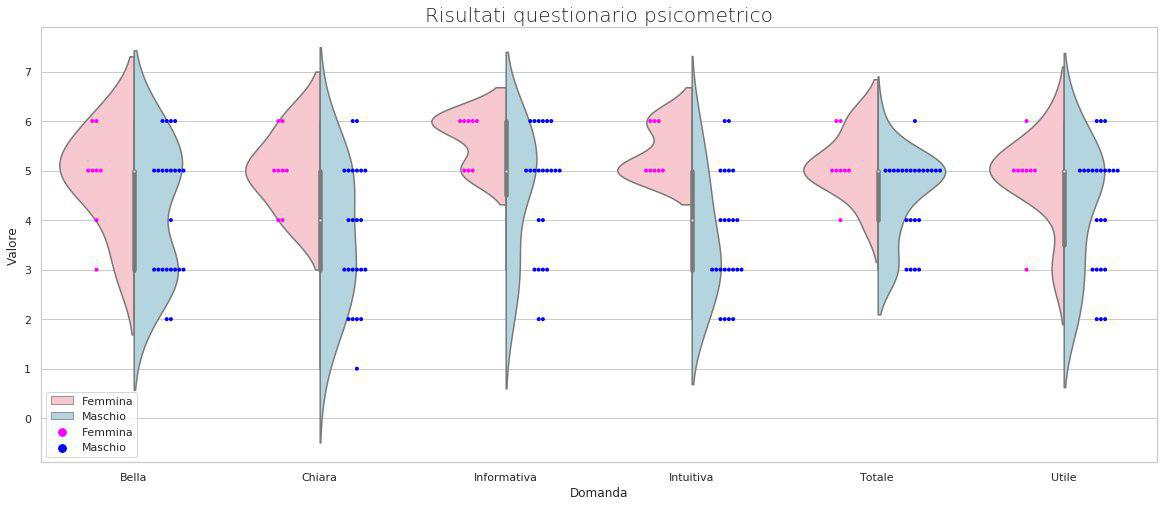
\includegraphics[width=\textwidth]{violin_plot_fm.jpg}
  \caption{Violin plot dei punteggi ottenuti al test divisi per sesso.}
  \label{plot:violin_fm}
\end{figure*}
È stata testata la facilità di lettura del grafico da parte di persone con problemi di discromatopsia grazie ad un pratico simulatore online\footnote{\url{https://www.color-blindness.com/coblis-color-blindness-simulator/}}.

Si nota subito dalla forma della distribuzione la presenza di code negative accentuate mentre i punteggi medi son sempre maggiori di 4 su 6.

Per testare in modo migliore l'efficienza del grafico, si son costruiti degli intervalli di confidenza \textit{binarizzando} i risultati, ovvero stabilendo la percentuale di voti ricevuti maggiori di una certa soglia (pari a 3, così da dividere le risposte in due parti uguali) e costruendo in seguito gli intervalli di confidenza.
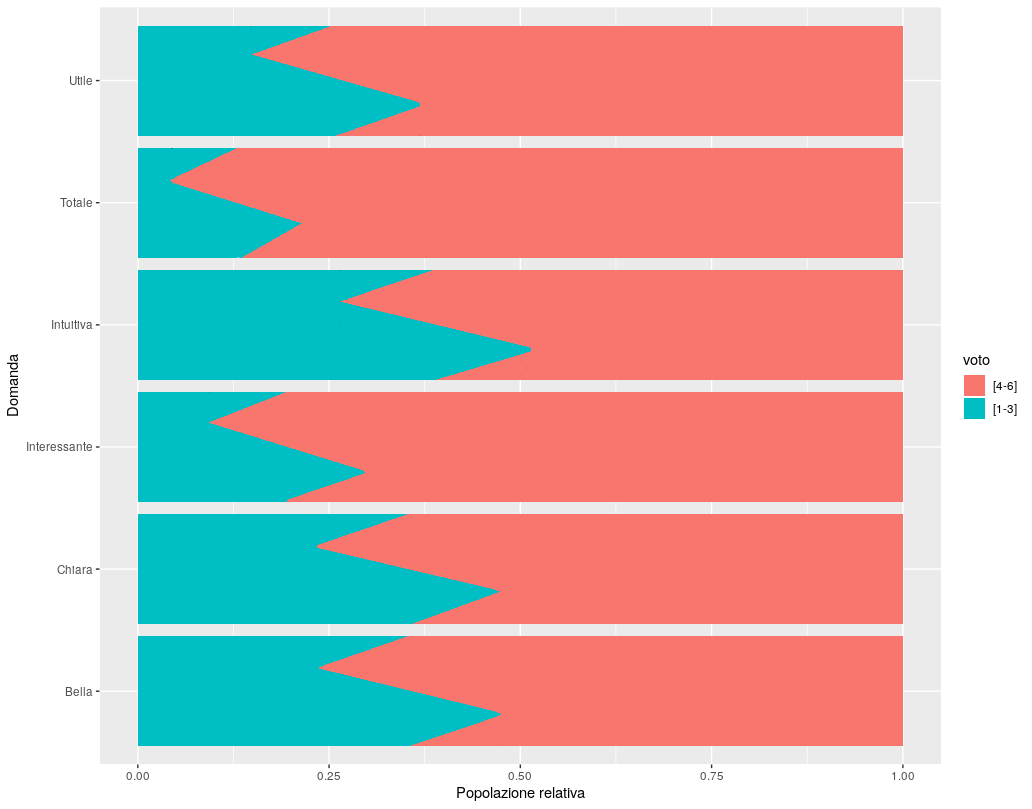
\includegraphics[width=\linewidth]{barplot.png}

Solo una variabile ha ricevuto tanti voti positivi quanti negativi: l'\textit{intuitività}, infatti come suggerito in seguito dai votanti stessi il grafico pare troppo ricco e complesso per essere intuitivo.
In tutti gli altri casi invece il punteggio ottenuto mostra che l'infografica nel complesso è stata apprezzata.

% correlogramma delle variabili: quali sono le più significative e quali sono collegate tra di loro
Inoltre è stata calcolata la correlazione tra i punteggi ottenuti al test per capire quali punti migliorare per offrire un prodotto migliore.
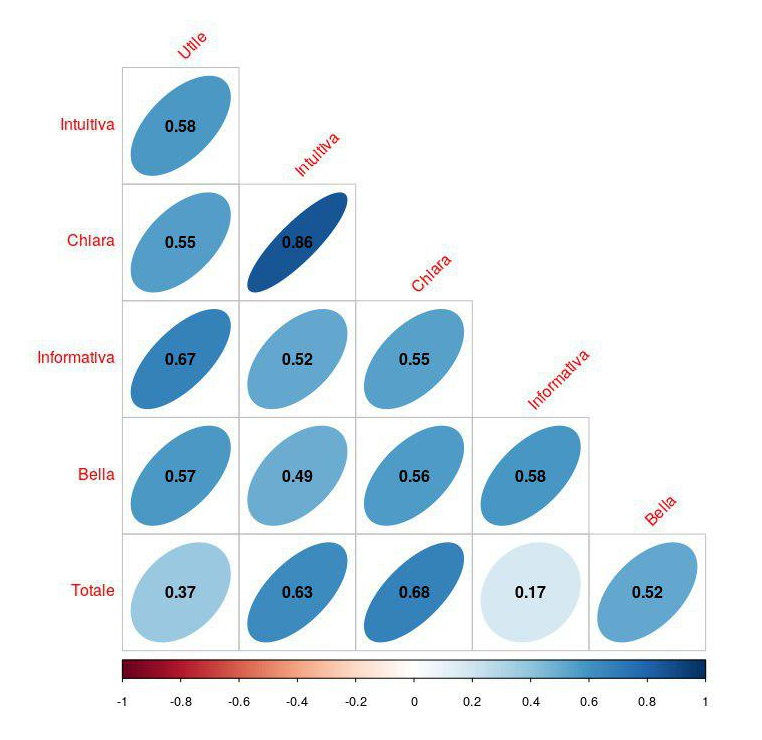
\includegraphics[width=\linewidth]{correlogramma.jpg}

Di particolare rilievo sono alcune coppie che offrono risultati particolarmente significativi.
% - chiarezza e intuitività: il grafico era poco chiaro perché poco intuitivo
Le variabili \textit{chiarezza} e \textit{intuitività} sono particolarmente legate: questo nesso può mostrare che il pubblico ha trovato poco chiaro il grafico perché poco intuitivo.
Intervistando in modo più dettagliato alcuni fruitori infatti è emerso che il primo grafico peccava in chiarezza in quanto conteneva troppe informazioni in troppo poco spazio; mentre nel secondo (il \textit{word cloud}) non tutti hanno compreso che la dimensione della parola fosse proporzionale alla frequenza del genere nei \textit{tweet}, obbligando quindi a inserire una rapida didascalia che lo esplicitasse.

% - il grafico ha ottenuto quel punteggio (5/6) perché chiaro
Tuttavia la variabile maggiormente legata al punteggio totale è la \textit{chiarezza}: il grafico deve gran parte del suo successo alla facilità di consultazione, dovuta principalmente dall'interattività con cui può essere consultato.
Infatti questa caratteristica è stata molto apprezzata dal pubblico, ed è stata ugualmente sfruttata per la consultazione.
% - totale e informativo: il grafico risulta essere molto informativo ma questo non implica un punteggio totale alto
Di scarso rilievo invece nella formazione del punteggio totale sono state l'\textit{informatività} e l'\textit{utilità}: il pubblico non ha apprezzato l'uso che se ne può fare del grafico o l'informazione contenuta, preferendo altre caratteristiche nella formulazione del giudizio complessivo.
Intervistando in modo più approfondito, è emerso che il pubblico sentiva un coinvolgimento maggiore quando era in grado di capire (intuitivamente o a seguito di ragionamento) l'informazione contenuta indipendentemente da quale questa fosse.

% conclusione: per migliorare il punteggio è opportuno aumentare l'intuitività, come constatato sono racchiuse troppe informazioni in troppo poco spazio
Dunque per migliorare l'efficienza del grafico è opportuno aumentarne l'intuitività, possibilmente togliendo alcune informazioni di scarso rilievo o rappresentandole in modo diverso, così da garantire la comprensione di un pubblico eterogeneo senza preparazione statistica.

\subsection{Tempo impiegato nella risposta alla domanda}
Ad un sottoinsieme (di cinque persone) degli intervistati è stata posta la seguente domanda: ``Qual è il secondo genere musicale più citato la mattina?'' così da testare il tempo di reazione.
I tempi variano dai 5 ai 30 secondi, e sono correlati alla preparazione statistica dell'individuo.
Infatti individui con una preparazione statistica, se pur minima, apprezzavano la chiarezza del grafico e lo trovavano di facile lettura, mentre al contrario chi non vanta una preparazione statistica ha trovato il grafico fortemente contro-intuitivo e di difficile lettura.

\subsection{Interviste non strutturate}
Ad un altro sottoinsieme (di tre persone) è stato chiesto di commentare il grafico in libertà, esponendo liberamente le proprie idee a riguardo.
Apprezzata l'interattività del primo e la semplicità del secondo, è emersa una problematica principale: solo un individuo (che vanta una preparazione statistica) ha capito cosa rappresentasse l'intervallo di confidenza posto nel barplot dei generi più citati nell'arco della giornata (sulla destra del primo grafico), rendendo necessario ripensare se e come rappresentarlo.

\hfill
\newpage
% \hfill
% \newpage
\part{Risultati e conclusioni}
% Quanti tweet abbiamo raccolto? Cosa abbiamo osservato? 
Il programma ha funzionato correttamente per tutto il breve periodo in cui la macchina virtuale è rimasta online, permettendo la raccolta di 2595 \textit{tweets}: nonostante il numero non sia particolarmente alto, è sufficiente per eseguire alcune analisi quali l'identificazione delle comunità.

\begin{figure}[h!]
  \centering
  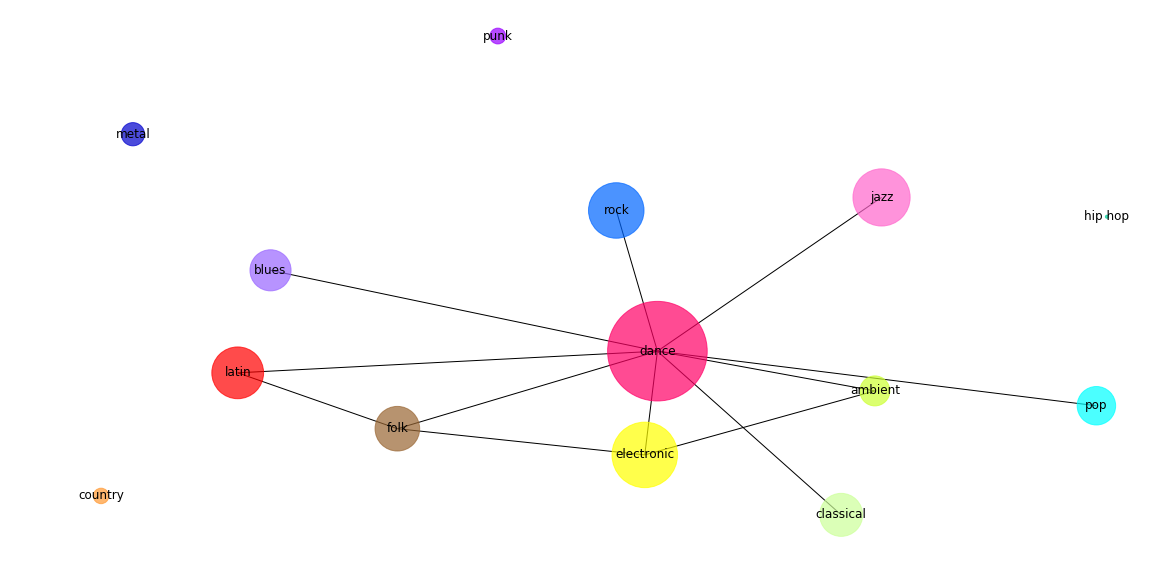
\includegraphics[width=\textwidth]{grafo.png}
  \caption{Grafo delle comunità rilevate dal programma durante il periodo in cui è rimasto online. La dimensione dei nodi è proporzionale al numero dei componenti.}
\end{figure}

% Quali dinamiche esistono tra le comunità e quali sono quelle più grandi?
Nonostante i tweet rappresentino la musica di cui si parla sul social e non quella ascoltata, si nota subito che non esistono comunità musicali particolarmente chiuse, se non in quattro casi.
Queste interagiscono col resto della piattaforma parlando principalmente della loro musica (presumibilmente preferita) e non di altri generi.
Queste quattro comunità sono le minori per dimensioni: probabilmente il loro isolamento è dovuto più al basso numero di \textit{tweet} raccolti che ad una tendenza delle persone che la compongono.
Al contrario, argomento di discussione comune alla maggior parte degli utenti è la musica \textit{dance}, tipica delle discoteche e di altri luoghi di ritrovo.
Il risultato mostra che gli utenti preferiscono discutere delle esperienze in comune piuttosto che del proprio genere preferito, rendendo difficile quindi una clusterizzazione tramite il contenuto dei loro messaggi.

%----------------------------------------------------------------------------------------
%	BIBLIOGRAPHY
%----------------------------------------------------------------------------------------

\hfill
\newpage
\printbibliography[title={Bibliografia e sitografia}]

%----------------------------------------------------------------------------------------

\end{document}
